\documentclass[UTF8]{ctexart}

\ctexset{
	section = {
		format+ = \zihao{4} \heiti \centering
	},
	subsection ={
		format+ = \zihao{-4} \heiti \raggedright
	},
	subsubsection = {
		format+ = \zihao{-4} \heiti \raggedright
	}
}
\pagestyle{empty}
\usepackage{float}
\usepackage{graphicx}
\graphicspath{{figures/}}
\usepackage{subfig}
\usepackage{appendix}
\usepackage{setspace}
\usepackage{url}
\usepackage{booktabs}
\usepackage{geometry}
\geometry{left=3.18cm,right=3.18cm,top=2.54cm,bottom=2.54cm}

\linespread{1.3}

\begin{document}
	
	%	\setlength{\baselineskip}{20pt}
	\zihao{-4} \songti
	
	\tableofcontents
	\newpage
	
	\section{问题重述}
	各国为控制疫情研发新冠疫苗。若干种疫苗需要顺序经过若干个工位生产。考虑到疫苗在不同工位生产的时间和顺序,我们需要根据疫苗生产的条件和要求,对不同环境的疫苗生产进行建模,以保证疫苗生产的高效性和有序性。
	
	首先疫苗生产有严格的限制条件:同一类型100剂疫苗为一箱进行处理;每种疫苗按照CJ1-CJ2-CJ3-CJ4的顺序在4个工位进行了加工;每个工位不能同时生产不同类型的疫苗,疫苗生产不允许插队,即进入第一个工位安排的每类疫苗的生产顺序决定整体生产顺序。其次有YM1-YM10等10种不同类型的疫苗需要生产。
	
	考虑以上影响因素,我们需要解决以下问题。
	
	\textbf{问题一:}
	对每箱疫苗在所有工位上的生产时间进行均值、方差、最值、概率分布等统计分析,掌握每个工位生产疫苗的能力水平。
	
	\textbf{问题二:}
	在最短时间内,生产YM1-YM10各100剂疫苗,建立数学模型,求出疫苗生产的顺序和生产总时间,并将结果填入表1。
	
	\textbf{问题三:}
	考虑疫苗实际生产时间的随机性。要求总时间比问题2给定的最短时间缩短5\%,建立数学模型,以最大的概率完成这个任务为目标,确定生产顺序,并给出缩短的时间比例与最大概率之间的关系。
	
	\textbf{问题四:}
	附件2中规定了不同规模的10种类型的生产任务。在每个每个工位每天生产的时间不能超过16小时和每种类型疫苗的生产任务不可以拆分的情况下,建立数学模型,使得可靠性为90\%,求出完成任务的最少天数。
	
	\textbf{问题五:}
	对于附件2中的疫苗生产任务,在生产时间限制在100天内、每个工位每天生产的时间不能超过16小时和每种类型疫苗的生产任务可以适当拆分的情况下,建立数学模型,安排生产计划,使得销售额达到最大值。
	
	\section{问题分析}
	\textbf{对问题一的分析:}问题一要对多组数据进行多种统计分析,考虑数据处理的方便性,我们先对数据进行预处理,采取部分数据确定其概率分布方式,再定义一个求取一组数据均值、方差、最值和确定分布方式的函数,最后使用函数对每组数据进行统计分析。
	
	\textbf{对问题二的分析:}问题二要制定疫苗的生产顺序和计算生产总时间。考虑到题目中的加工工位顺序和生产不允许排队的限制条件是非线性的,因此可以先用程序搜索出满足要求的可行的生产方案,从而解除非线性约束。根据可行的生产方案,我们采用启发式算法搜索最优解,即最短生产时间,并不断检查是否满足剩余的两项的限制条件,注意记录最优解的疫苗生产顺序。
	
	\textbf{对问题三的分析:}问题三要制定缩短时间下最大概率疫苗的生产顺序,以及给出缩短的时间比例与最大概率之间的关系。在问题二的基础上,将约束条件改成生产时间缩短5\%,用程序搜索满足对应的条件的可行方案,再采用启发式算法求最优解,但与问题二不同,最优解改成求最大概率,并注意记录最优解的疫苗产生顺序。启发式算法求最优解的过程,同样也是求最大概率与缩短时间的关系。
	
	\textbf{对问题四的分析:}
	
	
	\textbf{对问题五的分析:}
	
	
	\section{模型假设}
	为了简化问题,便于分析和求解,对模型进行以下合理的假设:
	\begin{enumerate}
		\item
	\end{enumerate}
	
	\section{定义和符号说明}
%	\begin{table}[!ht]
%		\caption{定义和符号说明表}\label{}
%		\begin{tabular*}{\hsize}{@{}@{\extracolsep{\fill}} c c}
%			\toprule[2pt]
%			符号 & 说明   \\
%			\hline
%			&    \\
%			&    \\
%			&    \\
%			\bottomrule[2pt]			
%		\end{tabular*}		
%	\end{table}
	\begin{table}[htbp]
		\centering
		\begin{tabular}{ c c }
			\toprule[2pt]
			符号 & 说明   \\
			\hline
			1 & 2  \\
			  &   \\
			  &   \\
			\bottomrule[2pt]
		\end{tabular}\caption{表格标题}\label{p1}
	\end{table}
	
	\section{模型建立、求解和分析}
	\subsection{问题一}
	\subsubsection{数据的正态性检验}
	\begin{itemize}
		\item 偏度和峰度
		\begin{enumerate}
			\item 偏度:描述数据分布不对称的方向及其程度
			
			当偏度≈0时,可认为分布是对称的,服从正态分布;
			
			当偏度>0时,分布为右偏,即拖尾在右边,峰尖在左边,也称为正偏态;
			
			当偏度<0时,分布为左偏,即拖尾在左边,峰尖在右边,也称为负偏态;
			
			\item 峰度:描述数据分布形态的陡缓程度
			
			当峰度≈0时,可认为分布的峰态合适,服从正态分布(不胖不瘦);
			
			当峰度>0时,分布的峰态陡峭(高尖);
			
			当峰度<0时,分布的峰态平缓(矮胖);
			
			\item Z分数(Z-score) 
			
			偏度Z-score=偏度值/标准误,峰度Z-score=峰度值/标准误。在$\alpha$=0.05的检验水平下,若Z-score在±1.96之间,则可认为资料服从正态分布。
			通过SPSS处理部分数据得到的结果如下图:	
%			\begin{figure}[h]
%				\centering %图片居中显示
%				\includegraphics{1_偏度与峰度}
%				\caption{偏度与峰度}
%			\end{figure}
		由图中数据计算可得可得Z-Scroe均处于±1.96之间,可认为四组数据均服从正态分布。			
		\end{enumerate}
		\item 图形判断
		\begin{enumerate}
			\item 直方图:表示连续性变量的频数分布,可以用来考察是否服从正态分布
			通过SPSS处理部分数据得到的结果如下图:
%			\begin{figure}[h]
%				\centering %图片居中显示
%				\includegraphics{1_偏度与峰度}
%				\caption{偏度与峰度}
%			\end{figure}
			\item P-P图和Q-Q图
			
			P-P图反映了变量的实际累积概率与理论累积概率的符合程度,Q-Q图反映了变量的实际分布与理论分布的符合程度。若数据点与理论直线(即对角线)基本重合,就认为数据服从正态分布。
			通过SPSS处理部分数据得到的结果如下图:
%			\begin{figure}[tbp]
%				\centering
%				\subfloat[Arabicnumerals]{\label{fig:a}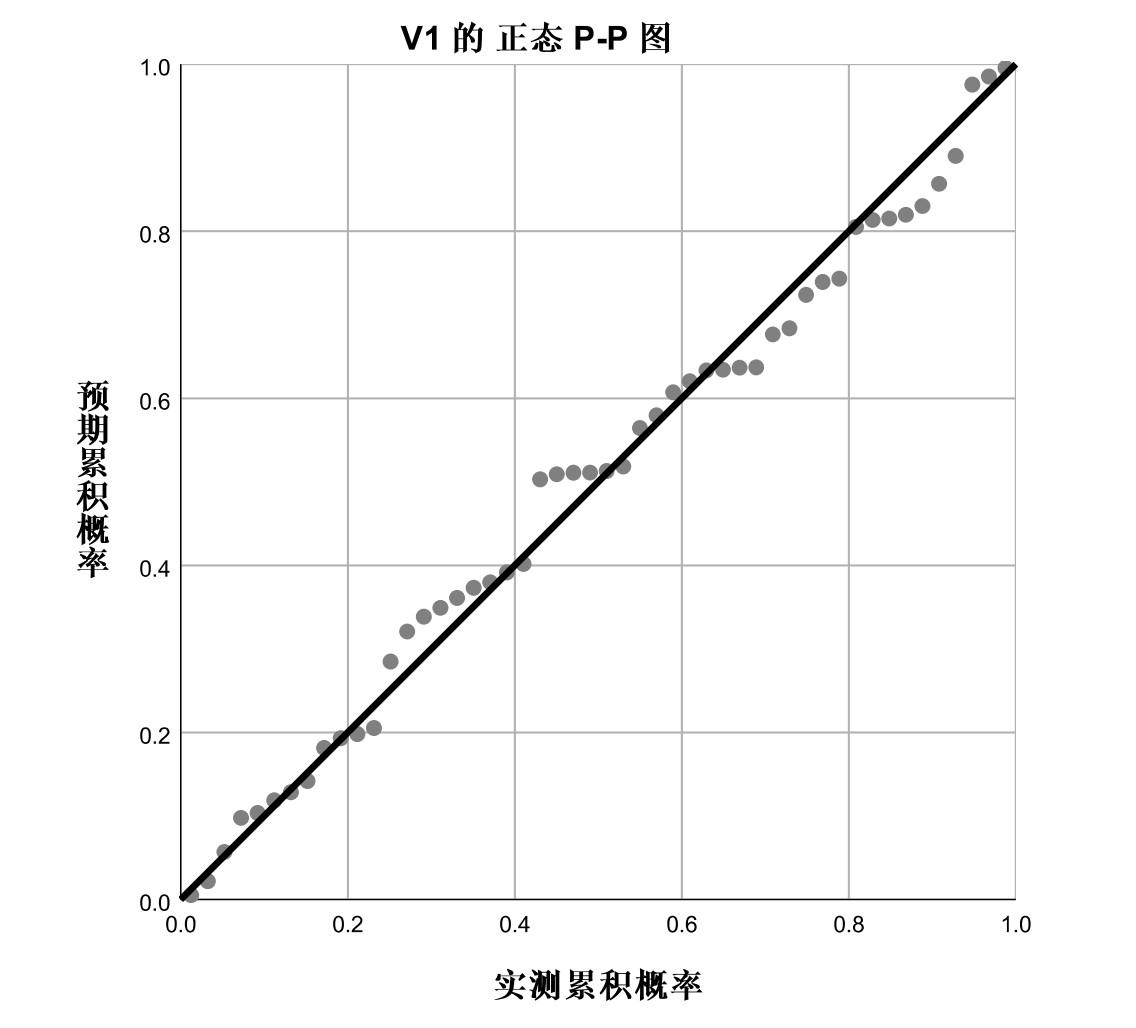
\includegraphics[width=1in]{1_pp}}\quad
%				\subfloat[Arabicnumerals]{\label{fig:b}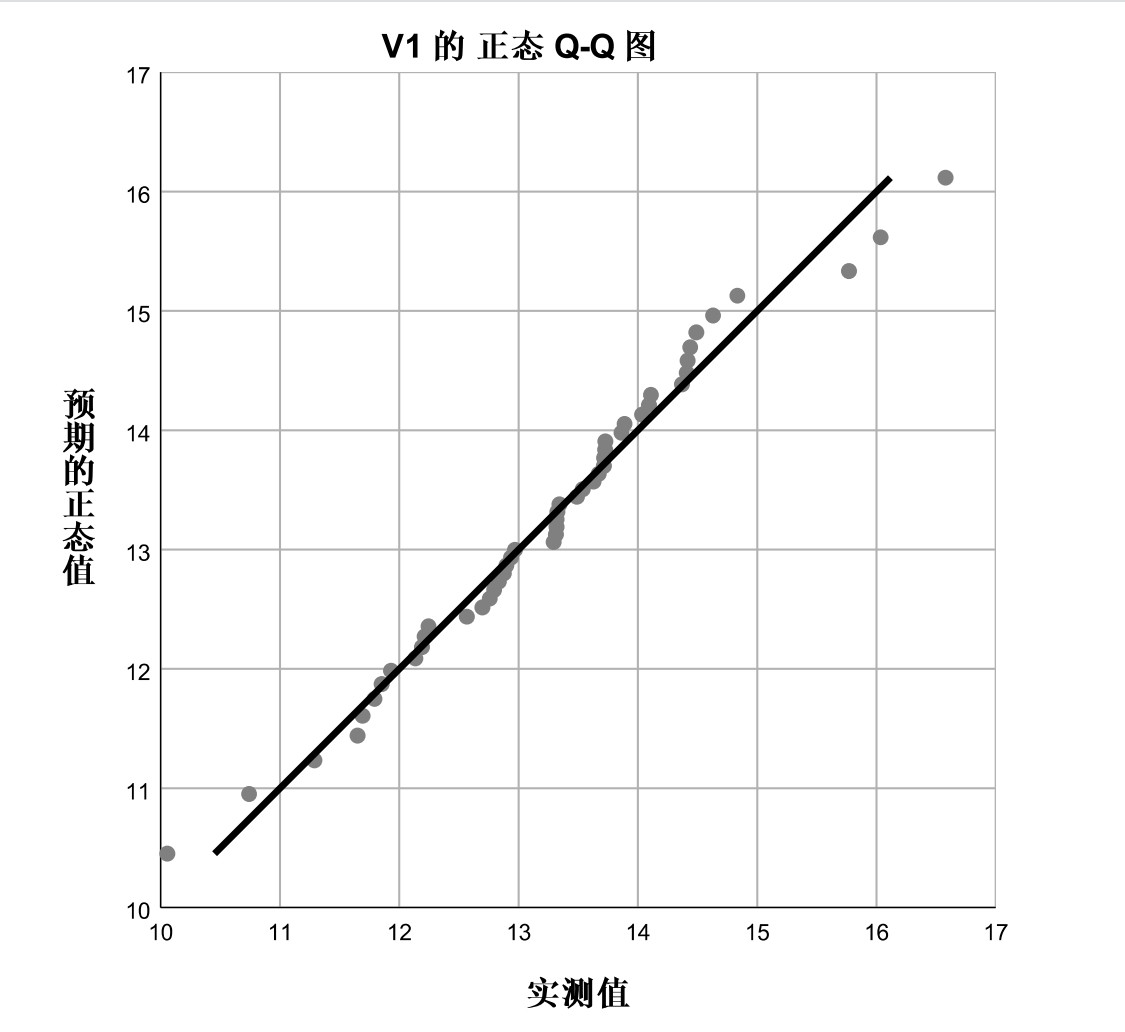
\includegraphics[width=1in]{1_qq}}\\	
%				\caption{}
%			\end{figure}
			
		\end{enumerate}
	\end{itemize}
	\subsubsection{模型求解}
		\begin{table}[!ht]
			\caption{工位CJ1的疫苗生产水平}\label{}
			\begin{tabular*}{\hsize}{@{}@{\extracolsep{\fill}}c|c|c|c|c|c|c|c|c|c|c }
				\toprule[2pt]
				      & YM1 & 	YM2 & 	YM3 & 	YM4 & 	YM5 & 	YM6 & 	YM7 & 	YM8 & 	YM9 & 	YM10  \\
				\hline
				
				均值  &      &       & 	  & 	  & 	  & 	   & 	  & 	  & 	 & 	 \\
				
				方差  &      &       & 	  & 	  & 	  & 	   & 	  & 	  & 	 & 	   \\
				
				最小值&      &       & 	  & 	  & 	  & 	   & 	  & 	  & 	 & 	  \\
				
				最大值&      &       & 	  & 	  & 	  & 	   & 	  & 	  & 	 & 	 \\
				\bottomrule[2pt]			
			\end{tabular*}
		\end{table}
		\begin{table}[!ht]
			\caption{工位CJ2的疫苗生产水平}\label{}
			\begin{tabular*}{\hsize}{@{}@{\extracolsep{\fill}}c|c|c|c|c|c|c|c|c|c|c }
				\toprule[2pt]
				& YM1 & 	YM2 & 	YM3 & 	YM4 & 	YM5 & 	YM6 & 	YM7 & 	YM8 & 	YM9 & 	YM10  \\
				\hline
				
				均值  &      &       & 	  & 	  & 	  & 	   & 	  & 	  & 	 & 	 \\
				
				方差  &      &       & 	  & 	  & 	  & 	   & 	  & 	  & 	 & 	   \\
				
				最小值&      &       & 	  & 	  & 	  & 	   & 	  & 	  & 	 & 	  \\
				
				最大值&      &       & 	  & 	  & 	  & 	   & 	  & 	  & 	 & 	 \\
				\bottomrule[2pt]			
			\end{tabular*}
		\end{table}
		\begin{table}[!ht]
			\caption{工位CJ3的疫苗生产水平}\label{}
			\begin{tabular*}{\hsize}{@{}@{\extracolsep{\fill}}c|c|c|c|c|c|c|c|c|c|c }
				\toprule[2pt]
				& YM1 & 	YM2 & 	YM3 & 	YM4 & 	YM5 & 	YM6 & 	YM7 & 	YM8 & 	YM9 & 	YM10  \\
				\hline
				
				均值  &      &       & 	  & 	  & 	  & 	   & 	  & 	  & 	 & 	 \\
				
				方差  &      &       & 	  & 	  & 	  & 	   & 	  & 	  & 	 & 	   \\
				
				最小值&      &       & 	  & 	  & 	  & 	   & 	  & 	  & 	 & 	  \\
				
				最大值&      &       & 	  & 	  & 	  & 	   & 	  & 	  & 	 & 	 \\
				\bottomrule[2pt]			
			\end{tabular*}
		\end{table}
		\begin{table}[!ht]
			\caption{工位CJ4的疫苗生产水平}\label{}
			\begin{tabular*}{\hsize}{@{}@{\extracolsep{\fill}}c|c|c|c|c|c|c|c|c|c|c }
				\toprule[2pt]
				& YM1 & 	YM2 & 	YM3 & 	YM4 & 	YM5 & 	YM6 & 	YM7 & 	YM8 & 	YM9 & 	YM10  \\
				\hline
				
				均值  &      &       & 	  & 	  & 	  & 	   & 	  & 	  & 	 & 	 \\
				
				方差  &      &       & 	  & 	  & 	  & 	   & 	  & 	  & 	 & 	   \\
				
				最小值&      &       & 	  & 	  & 	  & 	   & 	  & 	  & 	 & 	  \\
				
				最大值&      &       & 	  & 	  & 	  & 	   & 	  & 	  & 	 & 	 \\
				\bottomrule[2pt]			
			\end{tabular*}
		\end{table}
	
	\subsection{问题二}
	\subsubsection{模型建立}
	\subsubsection{模型求解}
	\subsubsection{模型分析}
	
	\subsection{问题三}
	\subsubsection{1}
	\subsubsection{2}
	\subsubsection{3}
	
	\subsection{问题四}
	\subsubsection{1}
	\subsubsection{2}
	\subsubsection{3}
	
	\subsection{问题五}
	\subsubsection{1}
	\subsubsection{2}
	\subsubsection{3}
	
	\section{模型评价}
	
	
	\section{参考文献}
	%	\begin{thebibliography}{9}%宽度9
	%		\bibitem{bib:one} ....
	%	\end{thebibliography}
	
	\section{附录}
	\begin{appendices}
		
	\end{appendices}
	
\end{document}